% !TeX root=../main.tex
\chapter{مفاهیم اولیه و پیش‌زمینه}
% ------------ Section 2.1
\section{دلایل و برتری‌های متن‌باز بودن قرارداد‌های هوشمند}
دلایل زیادی برای متن‌باز نوشتن قراردادهای هوشمند وجود دارد، در ادامه تعدادی از این دلایل توضیح داده می‌شود.

دلیل اول، بلاک‌چین‌ها
\gls{Confidentiality}
ندارند، همه‌ی نود‌های شبکه برای اجرای کد قرارداد هوشمند باید حداقل به
\glspl{bytecode}
قرارداد هوشمند دسترسی داشته باشند و این بایت‌کد‌ها در کاوشگرهای بلاکچین نیز وجود دارند، همچنین
\gls{Decompiler}هایی
وجود دارند که از بایت‌کد‌های قرارداد هوشمند کد سالیدیتی آن را به دست می‌آورند. پس در نتیجه تلاش برای مخفی کردن کدهای قرارداد هوشمند بیهوده خواهد بود.

دلیل دوم، اصلی‌ترین مذیت اپلیکیشن‌های غیرمتمرکز نسبت به اپلیکیشن‌های متمرکز عدم نیاز به اعتماد است، کاربرها می‌توانند کد‌های قرارداد هوشمند را بخوانند و به کد نوشته شده اعتماد کنند،‌در حالی که اگر کد برنامه برای همه کاربران قابل مشاهده نباشد کاربرها باید به سازندگان آن برنامه اعتماد کنند.

دلیل سوم، دیپلوی کردن قرارداد‌های هوشمند معمولاآسان نیست وسرعت تغییرات پایین‌تر از اپلیکیشن‌های متمرکز هست،‌ پس امکان این که با پیدا شدن هر مشکل بتوان به سرعت آن را درست کرد کمتر وجود دارد و مسئله امنیت بسیار اهمیت دارد. متن‌باز نوشتن قرارداد هوشمند باعث می‌شود چشم‌های بیشتری کدهای قرارداد را بخوانند و مشکلات احتمالی سریعتر مشخص و رفع شوند. تعداد زیادی از این پروژه‌ها از همان روز اول قرارداد هوشمند را به صورت متن‌باز توسعه می‌دهند، بعضی نیز ترجیح میدهند که پروژه به مرحله‌ای از توسعه برسد و سپس آن را متن‌باز میکنند.

ر این حوضه سرعت پیشرفت و توسعه به دلیل متن باز بودن به شدت بالاست به نحوی که در طی اجرای این پروژه مرج ریکوئستی روی کتابخانه OpenZeppelin زده شد که در همان روز مرج شد. این موضوع علاوه بر این که نشان‌دهنده سرعت پیشرفت بسیار بالاست، این موضوع را نیز نشان میدهد که در یک جامعه متن‌باز هر توسعه دهنده می‌تواند به پیشرفت جامعه به هر شکلی که می‌تواند کمک کند، اشکالاتی که مشاهده میکند را گزارش دهد یا تصحیح کند.

\begin{figure}[ht]
\centerline{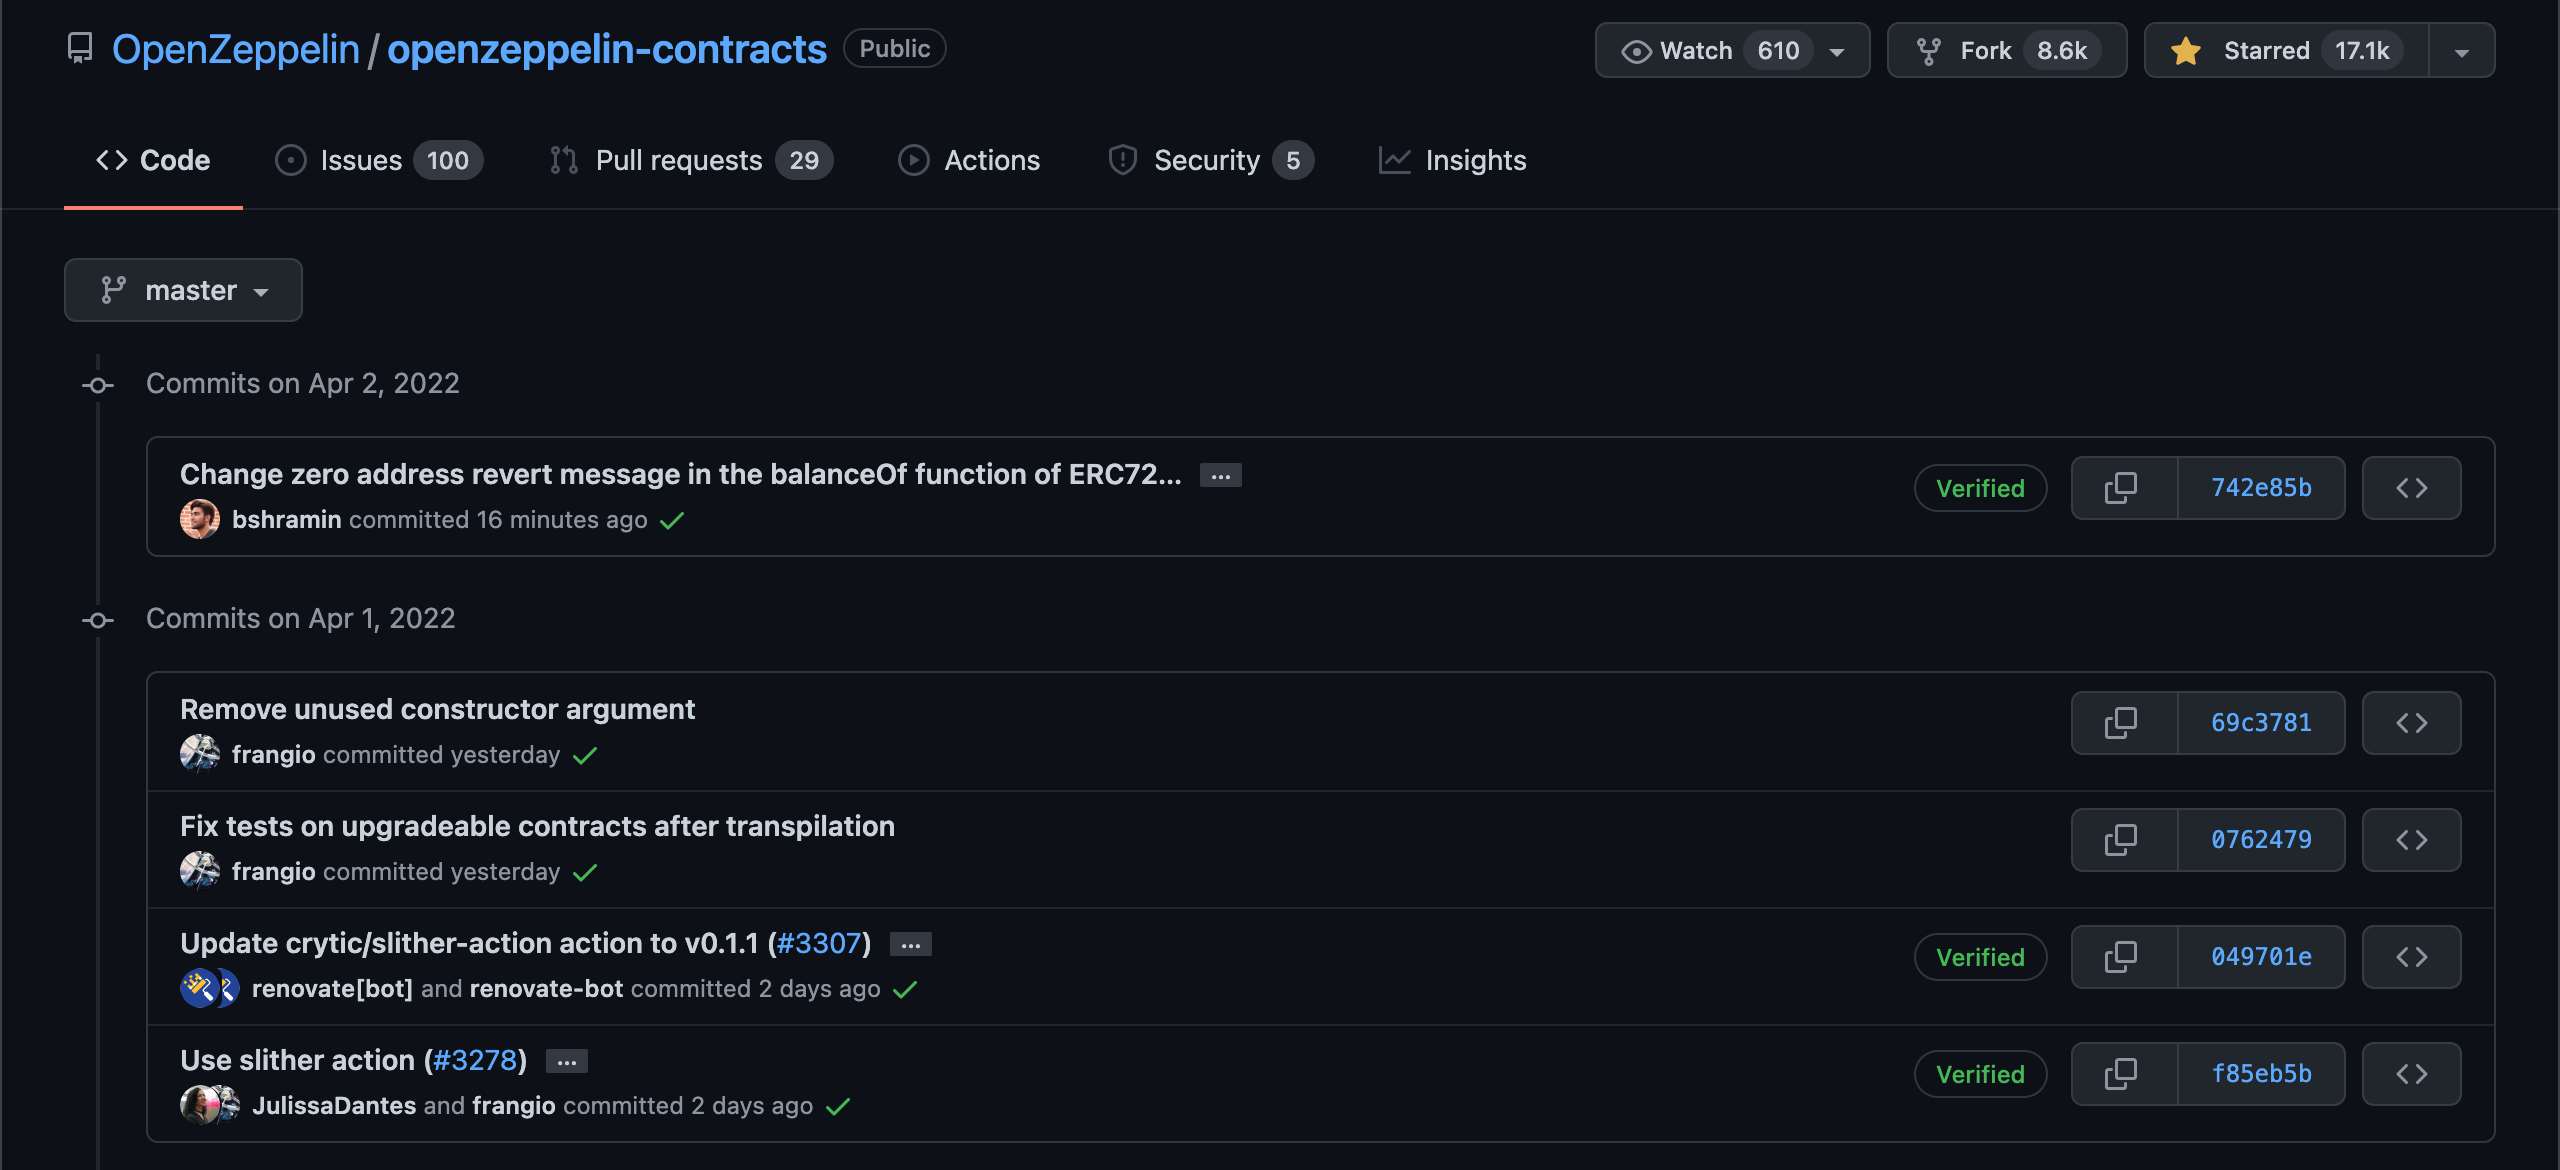
\includegraphics[width=15cm]{OpenZepplinContribution.png}}
\caption{در طی انجام پروژه مرج ریکوئستی روی OpenZeppelin باز شد که در همان روز مرج شد.}
\label{fig:zeppelin-merge-req}
\end{figure}







%\thispagestyle{empty} 
\section{مقدمه}
هدف از این فصل که با عنوان‌های  «مروری بر ادبیات موضوع%
\LTRfootnote{Literature Review}»،
«مروری بر منابع» و یا «مروری بر پیشینه تحقیق%
\LTRfootnote{Background Research}»
معرفی می‌شود، بررسی و طبقه‌بندی یافته‌های تحقیقات دیگر محققان در سطح دنیا و تعیین و شناسایی خلأهای تحقیقاتی است. آنچه را که تحقیق شما به دانش موجود اضافه می‌کند، مشخص کنید. طرح پیشینه تحقیق%
\LTRfootnote{Background Information}
یک مرور محققانه است و تا آنجا باید پیش برود که پیش‌زمینهٔ تاریخی مناسبی از تحقیق را بیان کند و جایگاه تحقیق فعلی را در میان آثار پیشین نشان دهد. برای این منظور منابع مرتبط با تحقیق را بررسی کنید، البته نه آنچنان گسترده که کل پیشینه تاریخی بحث را در برگیرد. برای نوشتن این بخش:
\begin{itemize}
	\item
	دانستنی‌های موجود و پیش‌زمینهٔ تاریخی و وضعیت کنونی موضوع را چنان بیان کنید که خواننده بدون مراجعه به منابع پیشین، نتایج حاصل از مطالعات قبلی را درک و ارزیابی کند.
	\item
	نشان دهید که بر موضوع احاطه دارید. پرسش تحقیق را همراه بحث و جدل‌ها و مسائل مطرح شده بیان کنید و مهم‌ترین تحقیق‌های انجام شده در این زمینه را معرفی نمائید.
	\item
	ابتدا مطالب عمومی‌تر و سپس پژوهش‌های مشابه با کار خود را معرفی کرده و نشان دهید که تحقیق شما از چه جنبه‌ای با کار دیگران تشابه یا تفاوت دارد.
	\item
	اگر کارهای قبلی را خلاصه کرده‌اید، از پرداختن به جزئیات غیرضروری بپرهیزید. در عوض، بر یافته‌ها و مسائل روش‌شناختی مرتبط و نتایج اصلی تأکید کنید و اگر بررسی‌ها و منابع مروری عمومی دربارهٔ موضوع موجود است، خواننده را به آنها ارجاع دهید.
\end{itemize}

\section{تعاریف، اصول و مبانی نظری}
این قسمت ارائهٔ خلاصه‌ای از دانش کلاسیک موضوع است. این بخش الزامی نیست و بستگی به نظر استاد راهنما دارد.

\section{مروری بر ادبیات موضوع}
در این قسمت باید به کارهای مشابه دیگران در گذشته اشاره کرد و وزن بیشتر این قسمت بهتر است به مقالات ژورنالی سال‌های اخیر (۲ تا ۳ سال) تخصیص داده شود. به نتایج کارهای دیگران با ذکر دقیق مراجع باید اشاره شده و جایگاه و تفاوت تحقیق شما نیز با کارهای دیگران مشخص شود. استفاده از مقالات ژورنال‌های معتبر در دو یا سه سال اخیر، می‌تواند به اعتبار کار شما بیافزاید.

\section{نتیجه‌گیری}
‌در نتیجه‌گیری آخر این فصل، با توجه به بررسی انجام شده بر روی مراجع تحقیق، بخش‌های قابل گسترش و تحقیق در آن حیطه و چشم‌اندازهای تحقیق مورد بررسی قرار می‌گیرند.	در برخی از تحقیقات، نتیجه نهایی فصل روش تحقیق، ارائهٔ یک چارچوب کار تحقیقی 
\lr{(research framework)}
است.